\documentclass{beamer}

\mode<presentation> {
\usetheme{Madrid}
\setbeamertemplate{footline}[page number]
\setbeamertemplate{navigation symbols}{}
}

\usepackage{graphicx}
\graphicspath{{figs/}}
\usepackage{booktabs}
\usepackage[short]{optidef}
\usepackage{tkz-graph}
\GraphInit[vstyle = Shade]
\tikzset{
  LabelStyle/.style = { rectangle, rounded corners, draw,
                        minimum width = 2em, fill = yellow!50,
                        text = red, font = \bfseries },
  VertexStyle/.append style = { inner sep=5pt,
                                font = \normalsize\bfseries},
  EdgeStyle/.append style = {->, bend left} }
\usetikzlibrary {positioning}
\definecolor{processblue}{cmyk}{0.96,0,0,0}
\definecolor{lightgray}{gray}{0.95}

\newcommand{\UNIT}{\texttt{UNIT}$(j,k)$}


\title[DNN and MILP]{Deep Neural Networks and Mixed Integer Linear Optimization}
\author{Authors: Mateo Fischetti, Jason Jo \\
Presented by: Guilherme Schardong, Luis Eduardo Craizer}
\date{\today}

\begin{document}

\begin{frame}
\titlepage
\end{frame}

\begin{frame}
\frametitle{Table of Contents}
\tableofcontents
\end{frame}

\section{Introduction}
\begin{frame}{Overview}
  \begin{itemize}
  \item Deep Neural Networks (DNN) are composed of layers of neurons
  \item Each neuron calculates an affine combination of the outputs of the previous layer;
  \item After combining the outputs, each neuron applies a non-linear operator on the result and feeds it to the next layer
  \end{itemize}
\end{frame}

\section{Definitions}
\begin{frame}{Definitions}
  \begin{itemize}
  \item A DNN is composed of $K+1$ layers, numbered $0$ to $K$
    \begin{itemize}
    \item Layer $0$ is a ``fake'' layer, and consists of the input of the network
    \item Layer $K$ is the output of the network
    \end{itemize}
  \item Each layer $k \in [0, K]$ is composed of $n_k$ neurons (or units), numbered from $1$ to $n_k$
  \end{itemize}
\end{frame}

\begin{frame}{Definitions}
  \begin{figure}
      \centering
      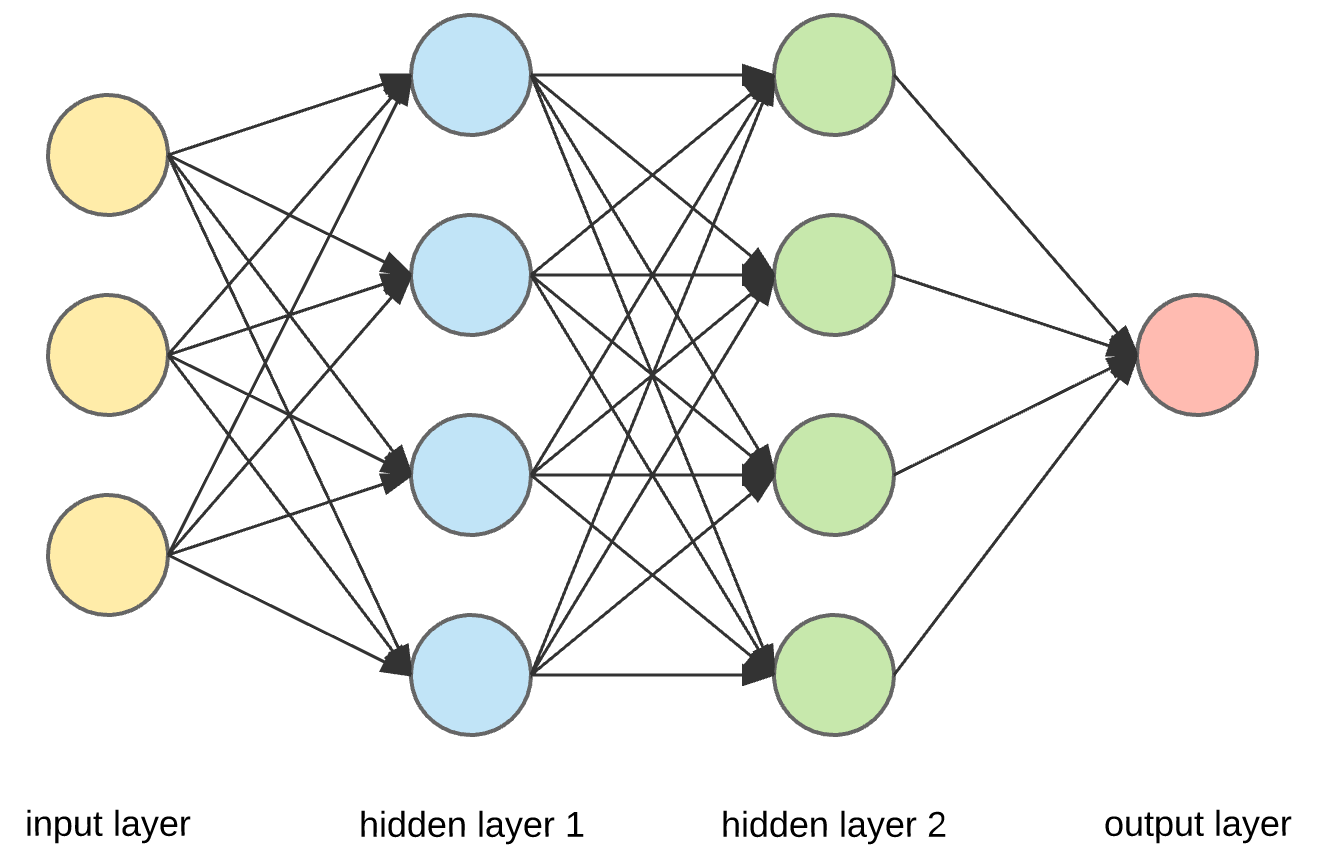
\includegraphics[width=\columnwidth]{dnn.png}
  \end{figure}
\end{frame}

\begin{frame}{Definitions}
  \begin{itemize}
  \item Let $x_k \in \mathbb{R}^{n_k}$ be the output vector of layer $k$, and $x_j^k$ is the scalar output of \UNIT
  \item For each layer $k \geq 1$, \UNIT \  computes its output using the following formula:

  $$
  x^k = \sigma(W^{k-1} x^{k-1} + b^{k-1})
  $$

  where $\sigma(.)$ is a non-linear function, $W^{k-1}$ and $b^{k-1}$ are a matrix of weights and a vector of activation biases resp.
  \end{itemize}
\end{frame}

\begin{frame}{Proposal}
  \begin{itemize}
  \item Use $W^k$ and $b^k$, $\forall k \in [0, K]$ to build an optimization model
    \begin{itemize}
    \item Applications in adversarial examples generation and activation visualization
    \end{itemize}
  \end{itemize}
  \pause
  \begin{block}{Problem}
    \centering
    $\sigma(.)$ is not linear
  \end{block}
\end{frame}

\begin{frame}{ReLU Operator}
  $$ \sigma(x) = \text{ReLU}(x) = \text{max}(0, x) $$
  \pause
  \begin{figure}[H]
    \centering
    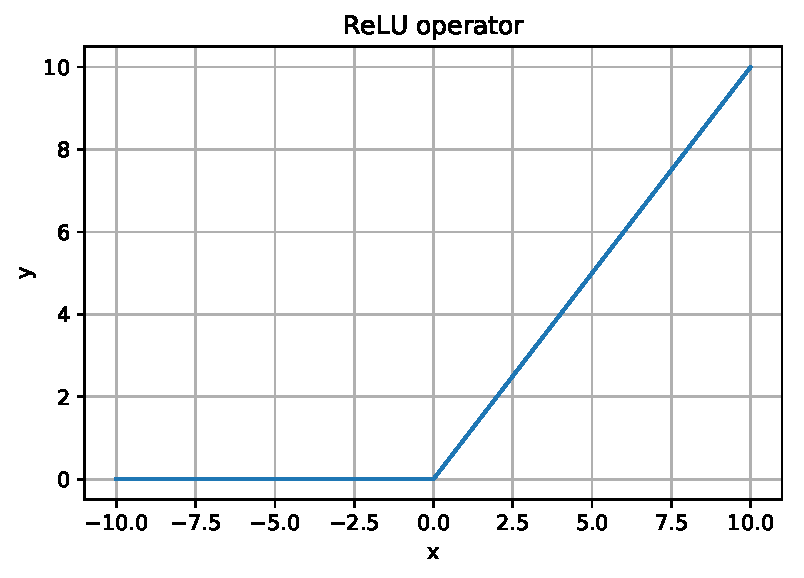
\includegraphics[width=0.8\columnwidth]{relu}
  \end{figure}
\end{frame}

\section{Model}

\begin{frame}
    \begin{itemize}
        \item It follows the basic scalar equation
        $$x = ReLU(w^T y + b)$$
        \item One can write the linear conditions
        $$w^T y + b = x - s,\ \ x \geq 0,\ \ s \geq 0$$
        to decouple the positive and negative  part of the ReLU input
        \item And we could add the
    bilinear condition $xs \leq 0$, making the solution unique.
    \end{itemize}
\end{frame}


\begin{frame}
    \begin{itemize}
        \item A second option is to introduce a binary activation variable $z$ and to impose the logical implications
        $$z = 1 \rightarrow x \leq 0$$
        $$z = 0 \rightarrow s \leq 0$$
        $$z \in \{0,1\}$$
        \item which are internally converted into proper linear inequalities of the type
        $$x \leq M^+(1-z)$$
        $$s \leq M^-z$$

    \end{itemize}
\end{frame}


\begin{frame}{Model}
  \begin{mini!}
  {x,z}{\sum_{k=0}^K \sum_{j=1}^{n_k} c_j^k x_j^k  + \displaystyle \sum_{k=1}^K \sum_{j=1}^{n_k} \gamma_j^k z_j^k}{}{}
  \addConstraint{\sum_{i=1}^{n_{k-1}} w_{ij}^{k-1} x_i^{k-1} + b_j^{k-1}}{= x_j^k - s_j^k \label{relu-1}}
  \addConstraint{x_j^k, s_j^k}{\geq 0 \label{relu-2}}
  \addConstraint{z_j^k}{\in \{0,1\}\label{relu-3}}
  \addConstraint{z_j^k = 1 \rightarrow x_j^k}{\leq 0 \label{relu-4}}
  \addConstraint{z_j^k = 0 \rightarrow s_j^k}{\leq 0}{\quad k = 1, \dots, K, j = 1, \dots, n_k \label{relu-5}}
  \addConstraint{lb_j^0 \leq x_j^0}{\leq ub_j^0}{\quad j = 1, \dots, n_0 \label{limits-xn0}}
  \addConstraint{lb_j^k \leq x_j^k}{\leq ub_j^k \label{limits-xnk}}
  \addConstraint{\overline{lb}_j^k \leq s_j^k}{\leq \overline{ub}_j^k}{\quad j = 1, \dots, n_k \label{limits-snk}}
  \end{mini!}
\end{frame}

\begin{frame}{Model discussion - feasibility}
  \begin{itemize}
  \item If the input is fixed (i.e. $lb_j^0 = ub_j^0, \forall j \in [1, n_0]$), all other variables have one possible value
  \item The binary variables $z_j^k$ are also defined uniquely, with a degenerate case when the ReLU unit receives a $0$ as input
  \item This makes it easy to find solutions for the model. Almost any random vector $x^0$ satisfies restriction~\ref{limits-xn0}
  \end{itemize}
\end{frame}

\begin{frame}{Model discussion - bound tightening}
  \begin{itemize}
  \item Bound tightening for $x$ and $s$ seriously improve the practical resolution of the model
  \item Modern MILP solvers define reasonable bounds for layer $0$ and propagate to layers $1 \dots K$
  \item A better option would be:
    \begin{enumerate}
    \item Scan the neurons of all hidden layers
    \item For each \UNIT, remove all constraints and variables from units on the same and subsequent layers
    \item Solve the resulting model twice: one to maximize $x_j^k$, other to maximize $s_j^k$
    \item The resulting optimal values can be used as bounds for $x_j^k$, and $s_j^k$
    \end{enumerate}
  \end{itemize}
\end{frame}

\section{Applications}
\begin{frame}{Applications}
  \begin{itemize}
  \item This model is unsuitable for training
  \item More suited for applications where the weights are fixed, and one wants to compute the best-possible input example
  \item Hence, overfitting the given DNN is actually a desired property
  \end{itemize}
\end{frame}

\begin{frame}{Experimental setup}
  \begin{itemize}
  \item Input: 28 x 28 hand-written digit figure
  \item 784 pixels normalized to gray-level [0, 1]
  \item 3 hidden layers with (8, 8, 8) ReLUs
  \item Last layer: 10 units to classify digits ``0'' to ``9''
  \item Number of epochs: 50
  \item Accuracy: 93.04\% on the test set
  \end{itemize}
\end{frame}

\begin{frame}{Feature visualization}
  \begin{itemize}
  \item We used our 0-1 MILP model to find input examples that maximize the activation $x_j^{k}$ of each \UNIT
  \item For our simple DNN, each of the resulting models could be solved within 1 second when using the bound strengthening procedure (described in the previous section)
  \end{itemize}
\end{frame}

\begin{frame}{Feature visualization}
    \begin{itemize}
        \item No nice visual pattern can be recognized (at least, for our DNN)
    \end{itemize}
  \begin{figure}
    \centering
    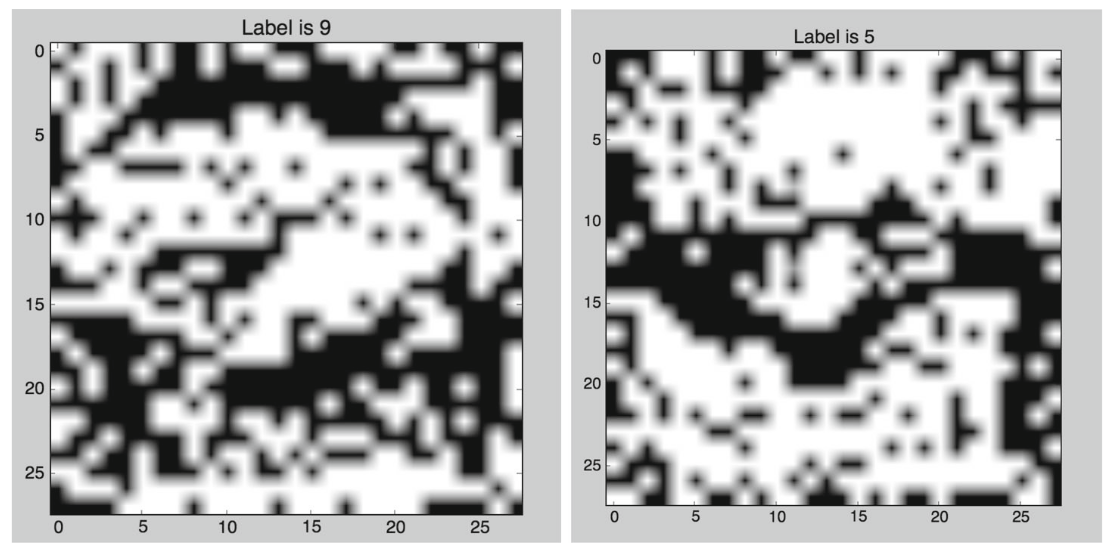
\includegraphics[width=0.9\columnwidth]{feature_visualization.png}
  \end{figure}
\end{frame}

\begin{frame}{Building adversarial examples}
  \begin{itemize}
  \item The problem here is to slightly modify a given DNN input so that to produce a wrong output
  \item We impose, in the final layer, that the activation of the required (wrong) digit is at least 20\% larger than any other activations
  $$x_{d+1}^{K} \geq 1.2 x_{j+1}^{K},\ \ \ \ \ \ j \in \{0, ..., 9 \} \backslash \{d \}$$
  \pause
  \item Similar constraints can be imposed to the input figure (e.g. maximum number of changed pixels in the input figure, or a maximum deviation of each pixel)
  $$-d_j \leq x_j^{0} - \widetilde{x_j^{0}} \leq d_j, \ \ d_j \geq 0, \ \ \ \ \mbox{for}\  j=1, ..., n_0$$
  \end{itemize}
\end{frame}

\section{Results}
\begin{frame}
  \begin{figure}
    \centering
    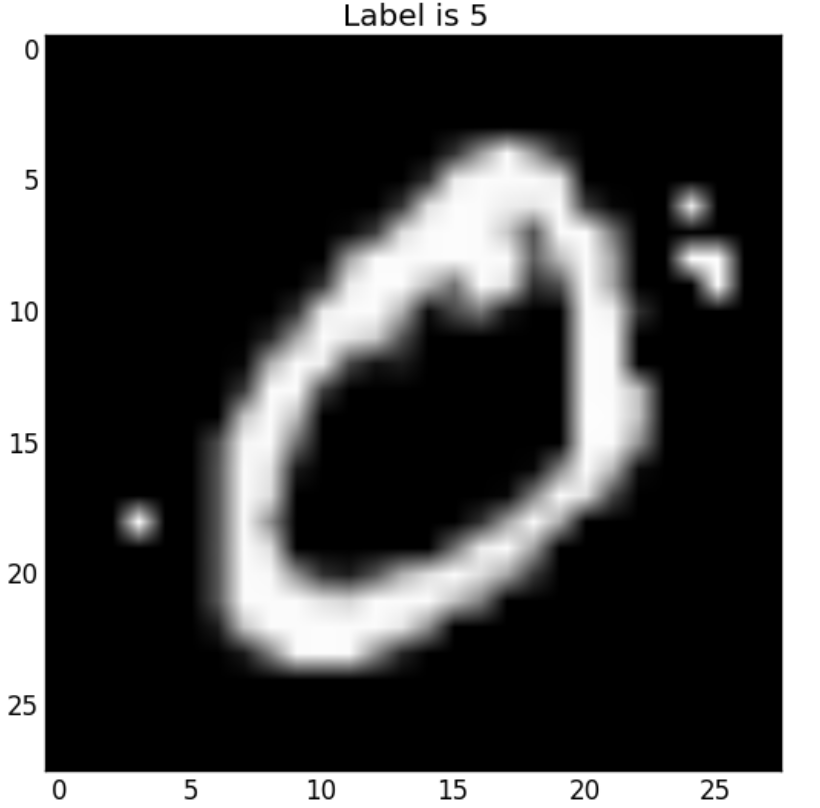
\includegraphics[width=0.48\columnwidth]{0-free.png}
    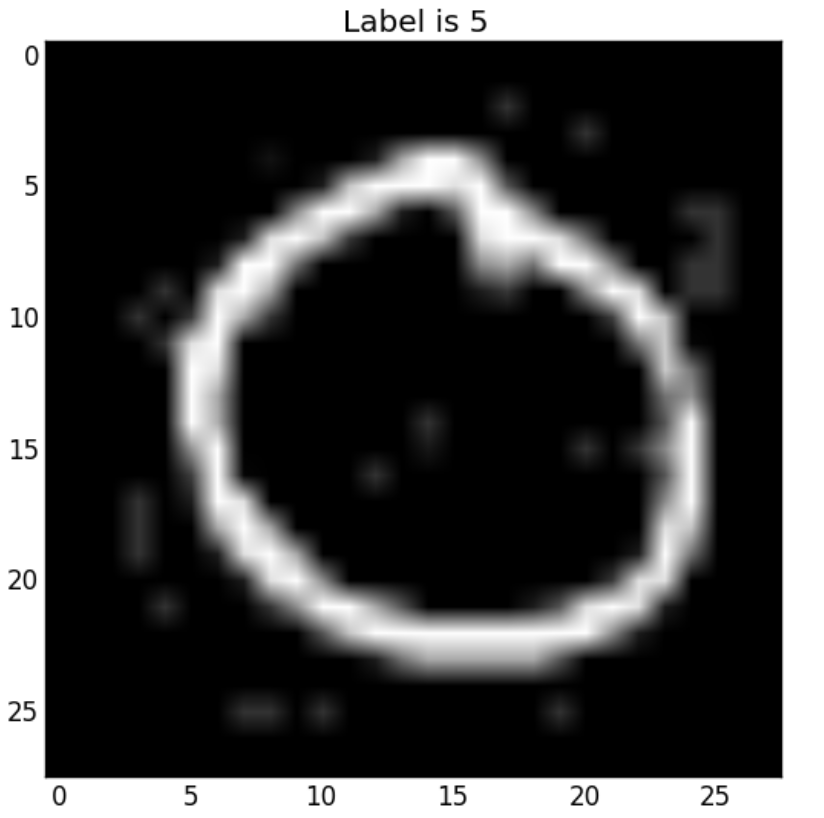
\includegraphics[width=0.48\columnwidth]{0-limited.png}
  \end{figure}
\end{frame}

\begin{frame}
  \begin{figure}
    \centering
    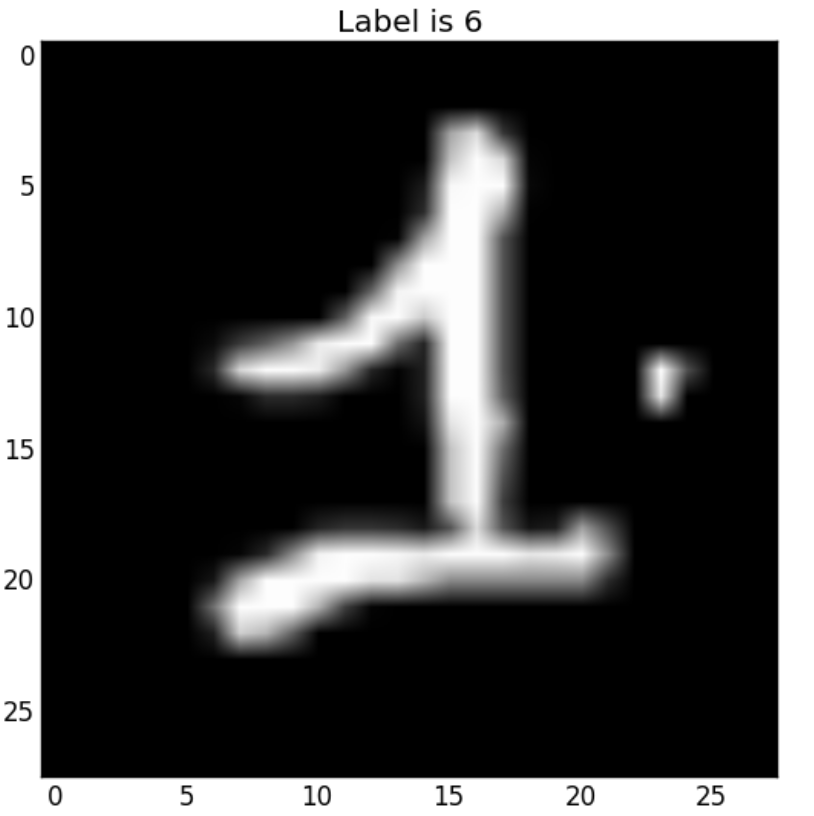
\includegraphics[width=0.48\columnwidth]{1-free.png}
    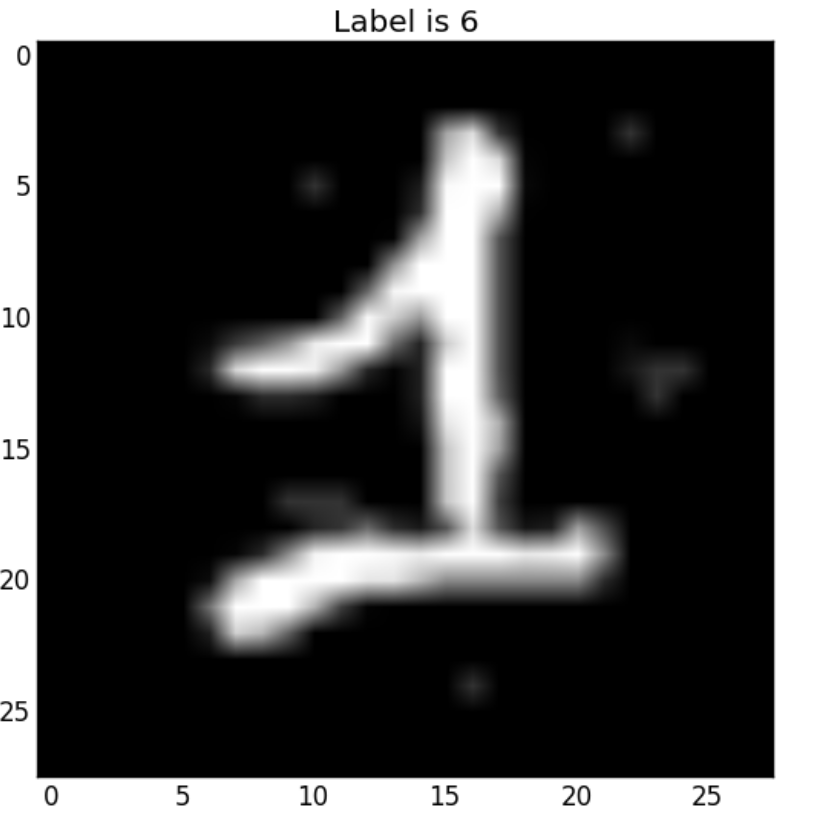
\includegraphics[width=0.48\columnwidth]{1-limited.png}
  \end{figure}
\end{frame}

\begin{frame}
  \begin{figure}
    \centering
    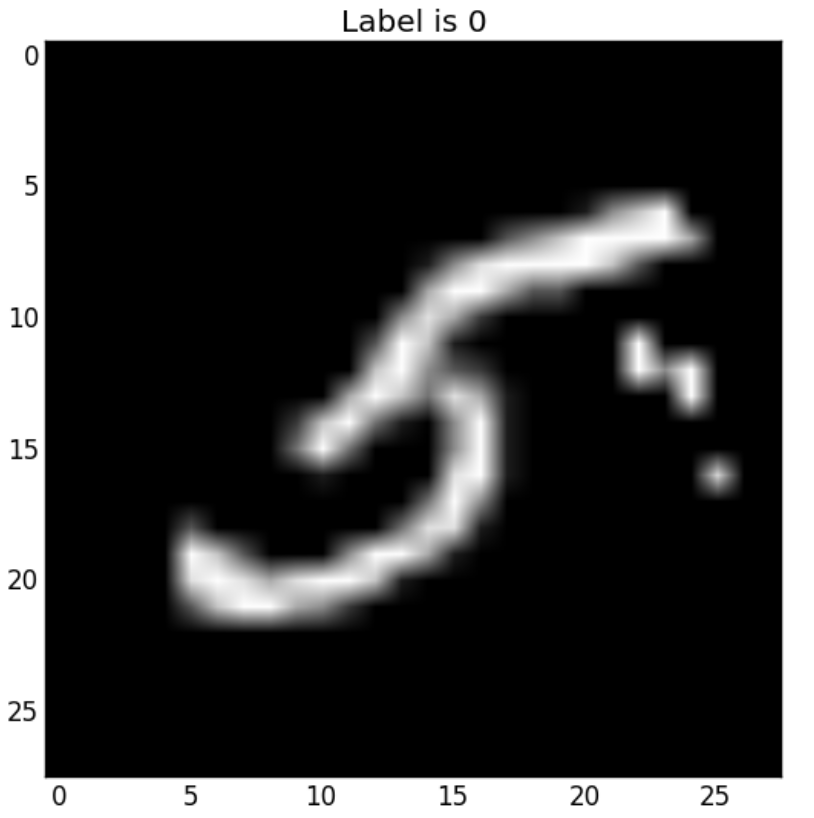
\includegraphics[width=0.48\columnwidth]{5-free.png}
    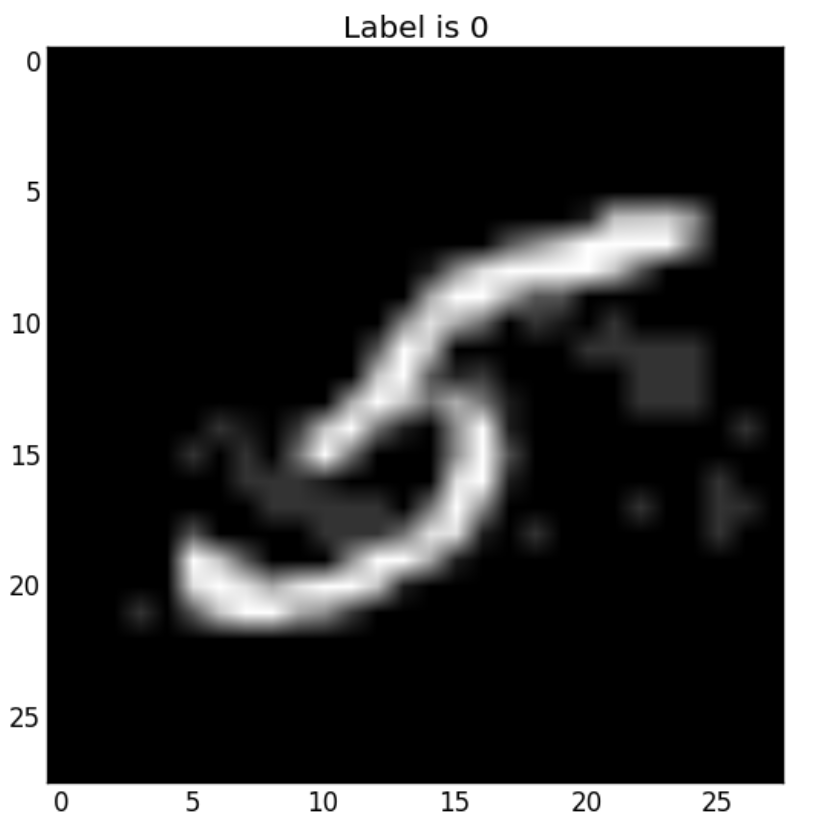
\includegraphics[width=0.48\columnwidth]{5-limited.png}
  \end{figure}
\end{frame}

\begin{frame}
  \begin{figure}
    \centering
    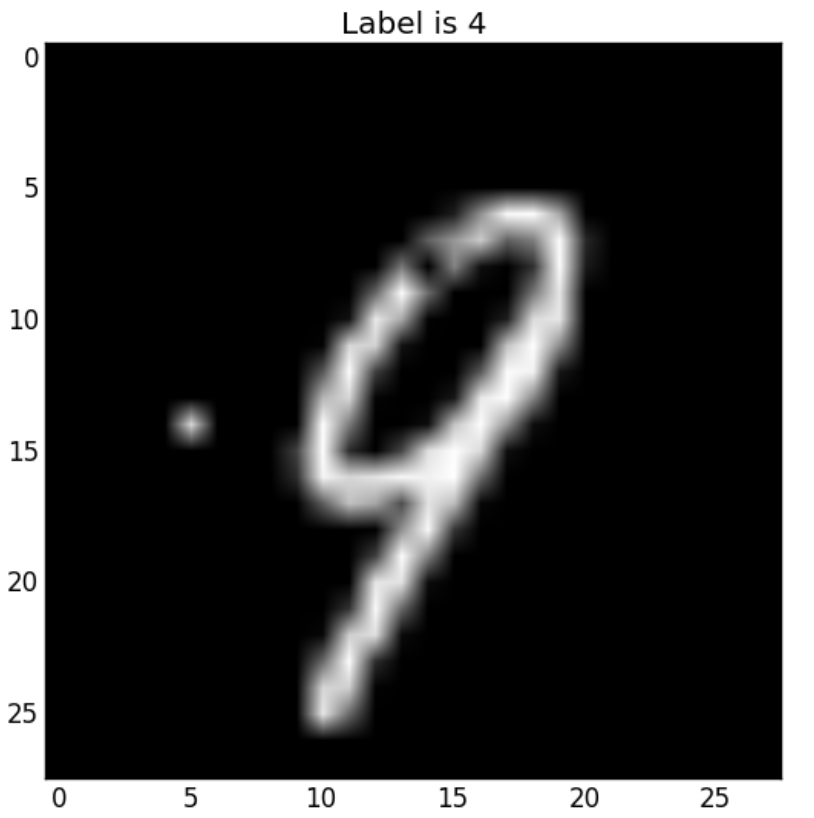
\includegraphics[width=0.48\columnwidth]{9-free.png}
    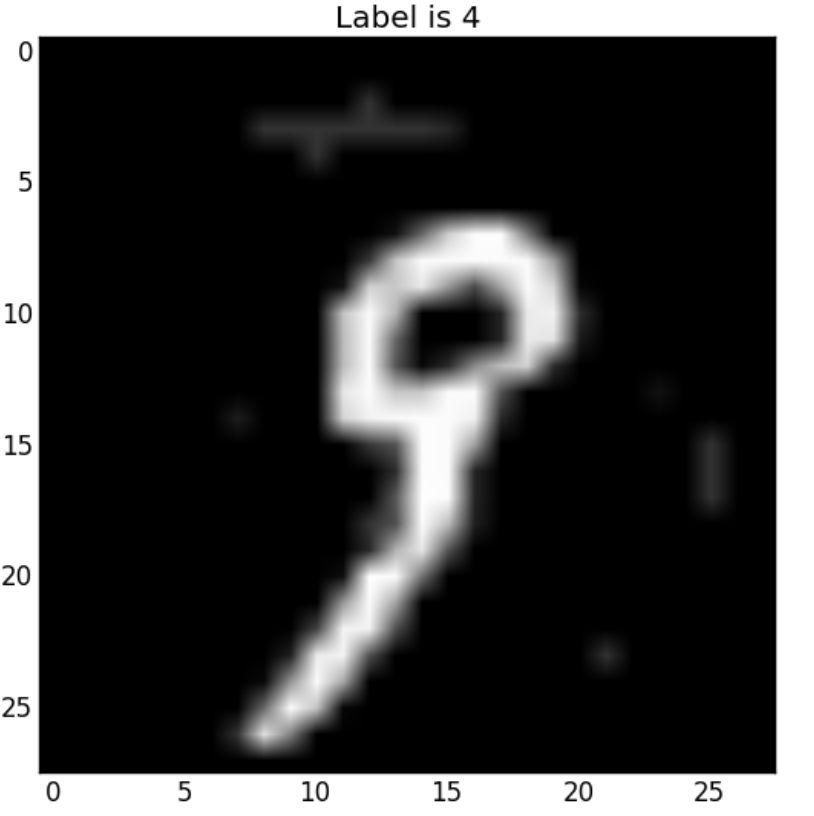
\includegraphics[width=0.48\columnwidth]{9-limited.png}
  \end{figure}
\end{frame}

\begin{frame}{Experimental setup}
  \begin{itemize}
  \item DNN1 - three hidden layers with eight units each
  \item DNN2 - six hidden layers with eight units each
  \item DNN3 - four hidden layers with (20, 10, 8, 8) units
  \item DNN4 - five hidden layers with (20, 10, 8, 8, 8) units
  \item DNN5 - six hidden layers with (20, 10, 10, 10, 10) units
  \end{itemize}
\end{frame}

\begin{frame}{Experimental setup}
  \begin{itemize}
  \item All networks were trained with $50$ epochs using Stochastic Gradient Descent
  \item The test accuracy was in the 93\%-96\% range
  \end{itemize}
\end{frame}

\begin{frame}{Basic vs. tight bounds}
  \begin{figure}
    \centering
    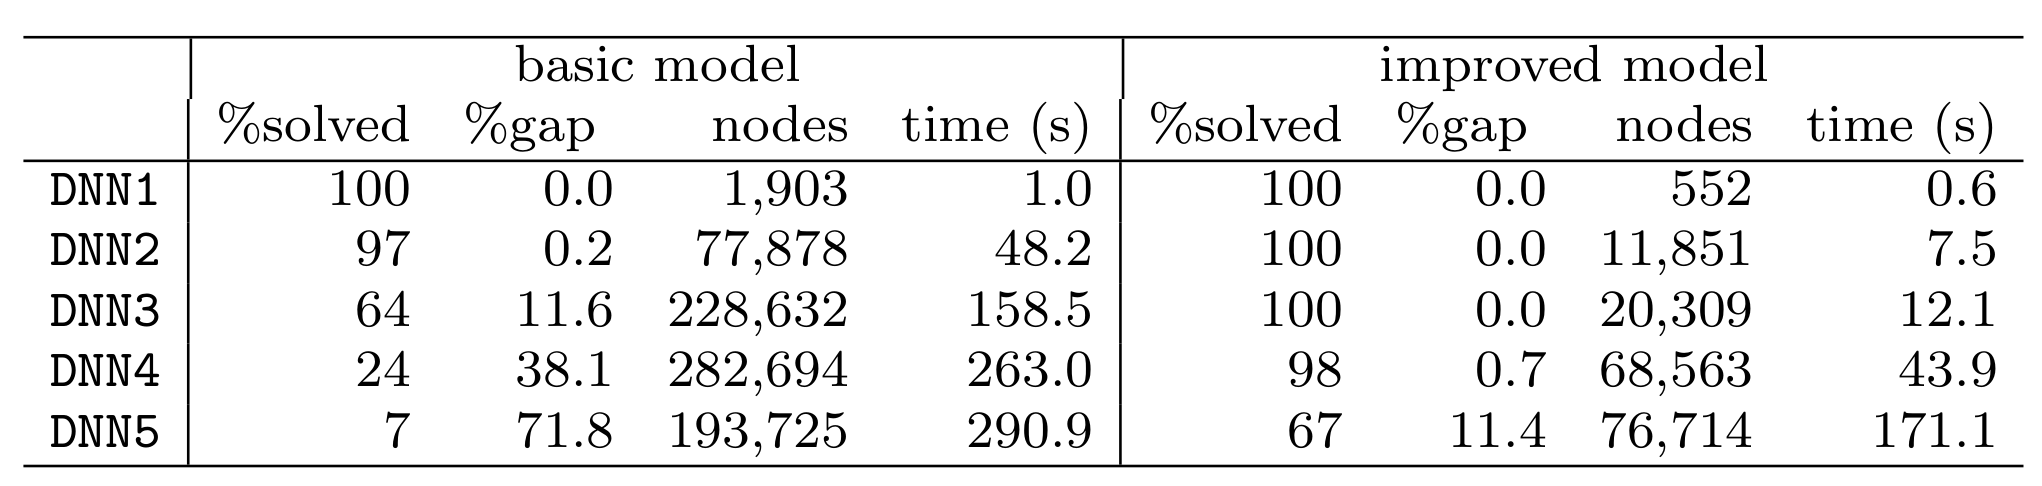
\includegraphics[width=\columnwidth]{tab-1.png}
  \end{figure}
\end{frame}

\begin{frame}{Exact tight bounds vs. weaker bounds}
  \begin{figure}
    \centering
    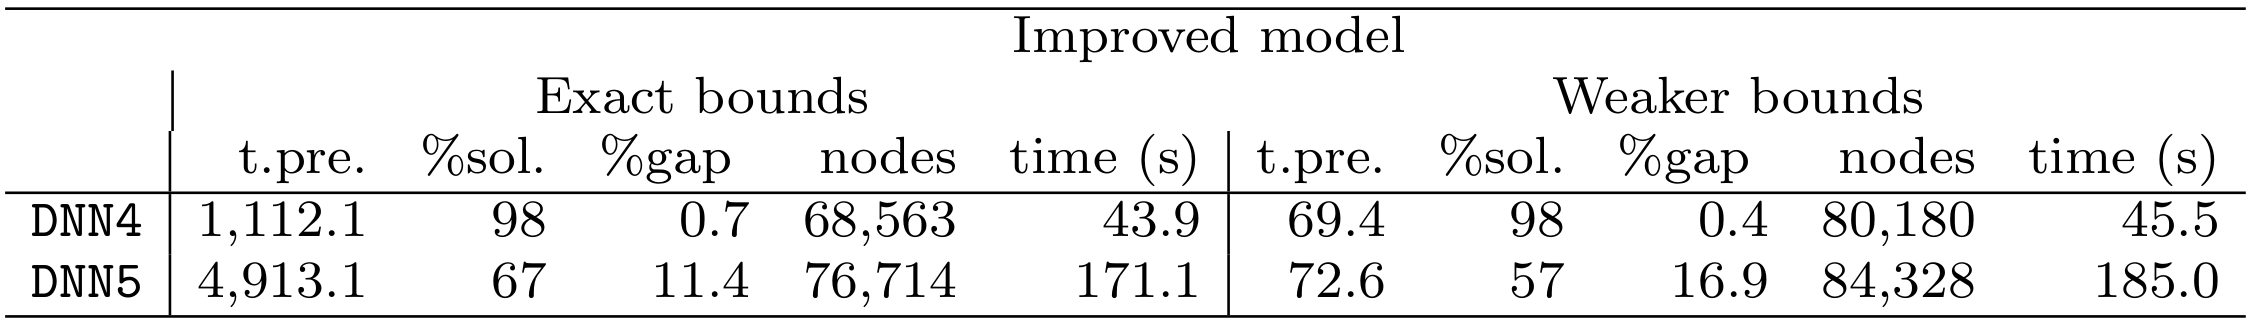
\includegraphics[width=\columnwidth]{tab-2.png}
  \end{figure}
\end{frame}

\begin{frame}{Basic vs. weaker bounds}
  \begin{figure}
    \centering
    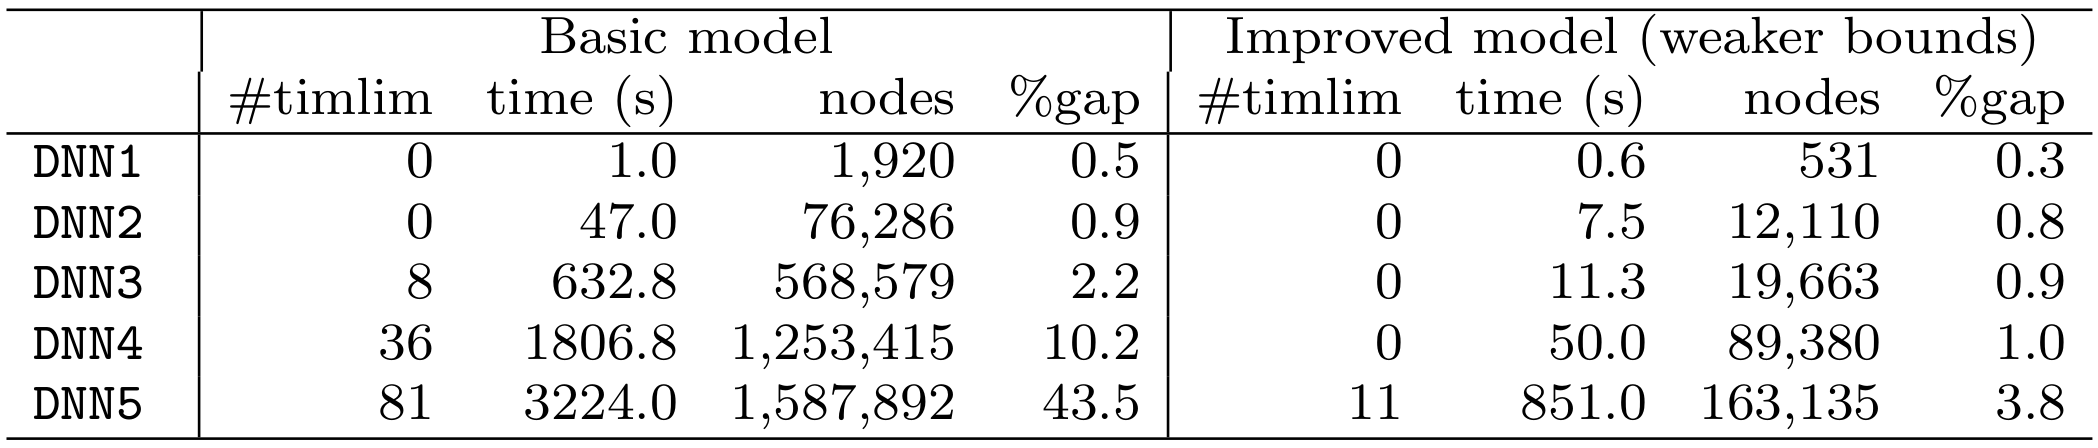
\includegraphics[width=\columnwidth]{tab-3.png}
  \end{figure}
\end{frame}

\section{Conclusions}
\begin{frame}{Conclusions}
  \begin{itemize}
  \item The formulation is good for constructing adversarial examples for trained DNNs
  \item Computing times still too large for reasonably sized networks, i.e. (30, 20, 10, 10, 10, 8, 8, 8)
  \item Future works: Extend to convolutional layers
  \end{itemize}
\end{frame}

\begin{frame}
  \Huge{\centerline{Thank you}}
\end{frame}

\end{document}